\chapter{Apprentissage automatique pour le traitement de la parole}
"La tristesse de l'intelligence artificielle est qu'elle est sans artifice, donc sans intelligence." 1987 -
Jean Baudrillard

\section{Apprentissage automatique : définitions}

Dans le domaine de l'intelligence artificielle (IA), l'apprentissage automatique (machine learning, abrégé ML en anglais) regroupe des méthodes permettant à un système d'apprendre un comportement. Généralement, l'apprentissage automatique permet, à partir de données plus ou moins massives, d'apprendre à caractériser de nouvelles données de même nature par une classification ou une régression. On dit alors qu'un système automatique a été entrainé avec des données d'entrainement (première étape) afin de permetre la prédiction des caractéristiques de nouvelles données similaires (seconde étape).

\subsection{Classification et régression}
La classification et la régression sont les deux grandes familles d'apprentissage automatique.
La classification correspond à résoudre un problème d'affectation de classes. Par exemple, on peut apprendre à un système de détecter la présence d'hippopotame au sein d'une image. Nous avons alors deux réponses possibles : la présence ou l'absence de l'animal. Ces réponses se transforment donc en classes, qui seront prédites par un apprentissage automatique de type classification. Nous avons donc un nombre défini et connu de catégories, donc un espace discret, qui sera utilisé par le système pour catégoriser chacune des données.

La régression quant à elle ne permet pas de catégoriser les données en classe, elle les inscrit dans un espace continu. Par exemple, on peut apprendre à un système de prédire la valeur d'un stock en bourses à partir des valeurs des jours précédents. Les réponses sont donc des nombres qui peuvent être positifs ou négatifs et qui ont une précision infinie. Nous avons donc une échelle de valeur dans laquelle le système va inscrire sa prédiction.

\begin{figure}
  \centering
  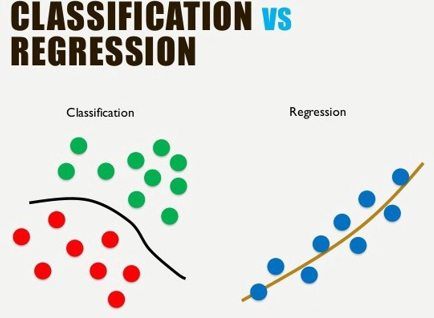
\includegraphics[width=8cm]{./Chapitre2/figures/classifVSreg.png}
  \caption{Représentation graphique de la classification et de la régression.}
  \label{fig:classifVSreg}
\end{figure}


Dans la figure~\ref{fig:classifVSreg}, on retrouve la différence graphique entre la classification et la régression. Pour une classification, le système automatique va chercher à mettre en place une démarcation entre les données de classes différentes, ici pour séparer les points verts et rouges. Tandis que pour une régression, le système va chercher la courbe qui minimise la somme des écarts de chaque point avec la courbe.

\subsection{Les facteurs de l'apprentissage automatique}
Un des facteurs les plus important pour la qualité de ces systèmes automatiques ce sont les données d'entrainement. Plus elles sont qualitatifs, c'est-à-dire qu'elles sont les pus proches des données réelles que nous voulons analyser, et plus le système sera performant dans sa tache de prédiction. Mais la qualité ne fait pas tout dans ce contexte, la quantité et l'exhaustivité sont tout aussi importantes.

Mais les données ne font pas tout, le choix de l'algorithme mis en place pour apprendre le système automatique est tout aussi important. Il existe de nombreuses méthodes mathématiques permettant de modéliser un système automatique. Ces derniers sont communément divisés en deux groupes, les méthodes d'apprentissage automatique et les méthodes de réseaux de neurones, appelé Deep Neural Network en anglais (DNN).
Le choix des données et du modèle est donc la principale question à se poser lorsque nous mettons en place des apprentissages automatiques.

Ces choix doivent être en adéquation avec le type de caractérisation recherché. En effet, il existe deux principaux types d'apprentissage : l'apprentissage supervisé et l'apprentissage non-supervisé.

\subsection{Apprentissage supervisé et non supervisé}

\begin{figure}
  \centering
  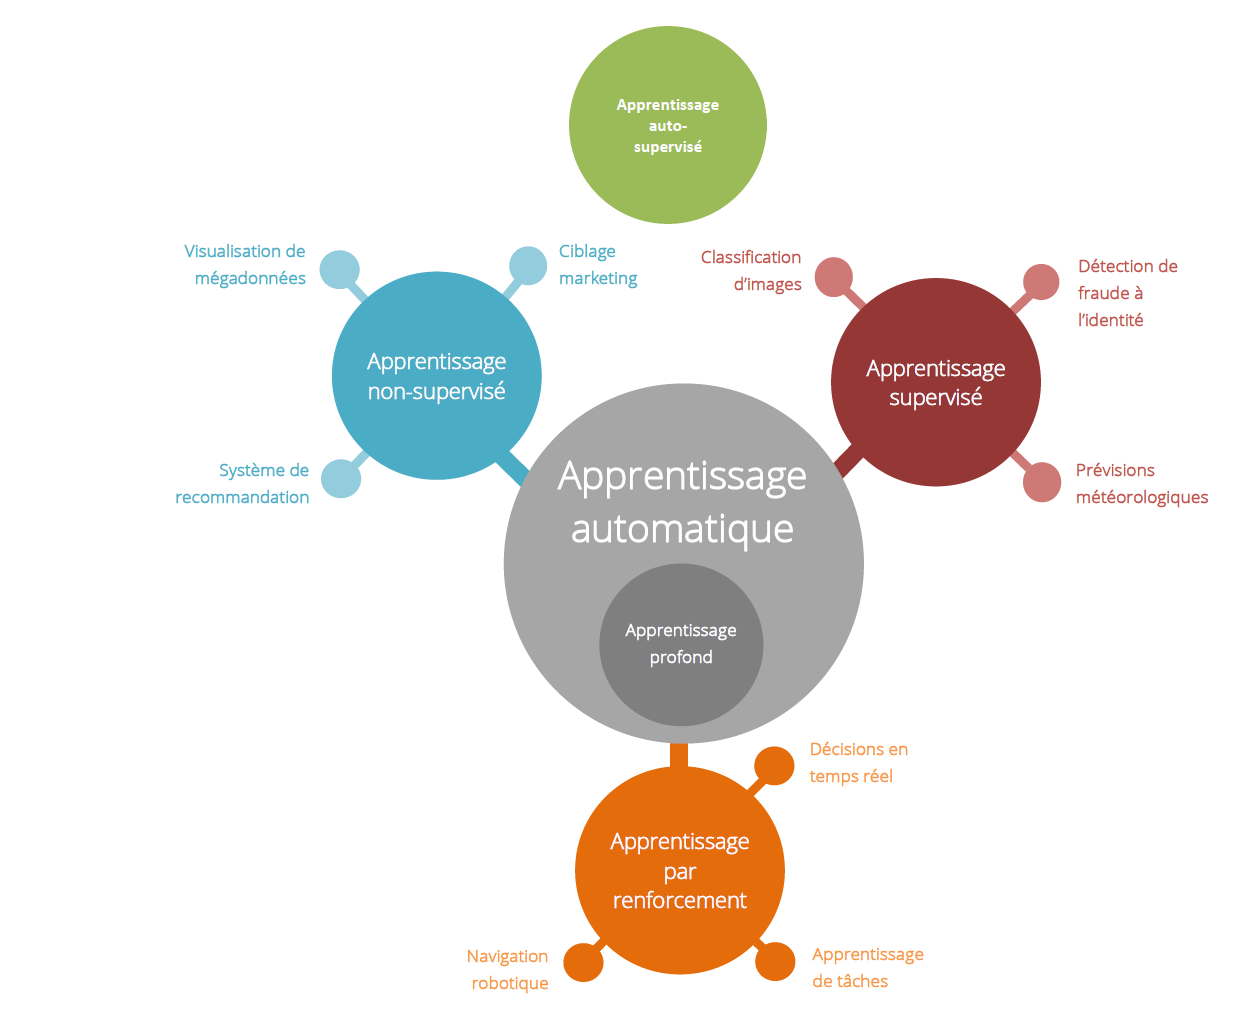
\includegraphics[width=.95\textwidth]{./Chapitre2/figures/typeApprentissage.png}
  \caption{Les différents types d'apprentissage et des exemples d'utilisation.}
  \label{fig:typeApprentissage}
\end{figure}

Il existe de nombreux type d'apprentissage dont les principaux sont présentés dans la figure~\ref{fig:typesApprentissage}. Dans le contexte de cette thèse, nous ne parlerons que d'apprentissage supervisé, non supervisé et auto-supervisé.

Lorsque nous parlons d'apprentissage supervisé, nous connaissons déjà les sorties souhaitées pour nos données d'entrainement. Nous avons une référence pour chaque document contenu dans les données d'entrainement et nous apprenons au système à retrouver ces références.
Il y a plusieurs mots pour définir ces références, on peut parler d'étiquettes, d'annotation ou de label. Ce type d'apprentissage ne peut donc être mis en place que lorsque nous avons des données d'entrainement qui sont annotées soit par l'humain soit automatiquement par un autre système d'apprentissage ou par un ensemble de règle par exemple. L'apprentissage supervisé peut être soit une classification, soit une régression.

Tandis que pour l'apprentissage non supervisé, nous ne connaissons pas les sorties attendues pour nos données d'entrainement. L'objectif du système automatique est donc de proposer une caractérisation des données d'entrée, en se basant sur des comparaisons entre ces dernières. Par exemple, on peut détecter la présence d'un hippopotame dans des images sans pour autant avoir des données annotées. Nous spécifions le nombre de classe au système et il va essayer d'apprendre tout seul ce qui différencie les images en entrée, ici la présence ou l'absence de l'animal. L'apprentissage non supervisé peut également servir à prédire une régression.

Un nouveau type d'apprentissage est de plus en plus utilisé, notamment dans le domaine de traitement des langages naturels (TALN), c'est l'apprentissage auto-supervisé, self supervised learning en anglais (SSL). Il s'agit d'un apprentissage où l'on n'a pas d'étiquette pour nos données d'apprentissage. Pour compenser leur absence, on prend une très grande masse de données et on en cache une partie. Le système devra alors retrouver les parties cachées à partir des parties disponible. Ainsi le système crée à la volée des étiquettes qui lui permettront d'apprendre.
Cette technique est utilisé par exemple dans la traduction de texte, où l'on apprend à représenter deux langues différentes puis en comparant ces deux représentations, on est capable de passer d'une langue A à une langue B sans avoir fourni au système des traductions d'un document de la langue A vers la langue B.

\textcolor{red}{est ce que je détaille l'apprentissage par renforcement?}

\section{Quelques familles d'apprentissage automatique}
Dans le contexte de la reconnaissance d'émotion, de nombreuses méthodes d'apprentissage automatique sont utilisées, que ce soit pour faire de la claissification lorsque l'on considère une émotion comme discrète ou de la régression quand on considère une émotion comme continue.
%https://tel.archives-ouvertes.fr/tel-02479126/document
%https://tel.archives-ouvertes.fr/tel-02925116/document


% a) Introduction (principe de base et familles des ML et protocoles expérimentaux)
% b) Les types d'apprentissage
%     1. Supervisée
%     2. Non supervisée
%     3. Auto supervisé
% c) Définition du DNN
%     1. Du perceptron au multi couche
%     2. Algorithme d'apprentissage
%     3. L'initialisation et ses enjeux
%     4. Les régularisations
% d) Dans le cadre du traitement de la parole
%     1. Quels sont les spécificités du traitement de la parole (speech => text)
%     2. Archi : CNN, RNN (donc lstm) et donc maintenant c'est les pre-train qui emergent
